\section{RAID einrichten}
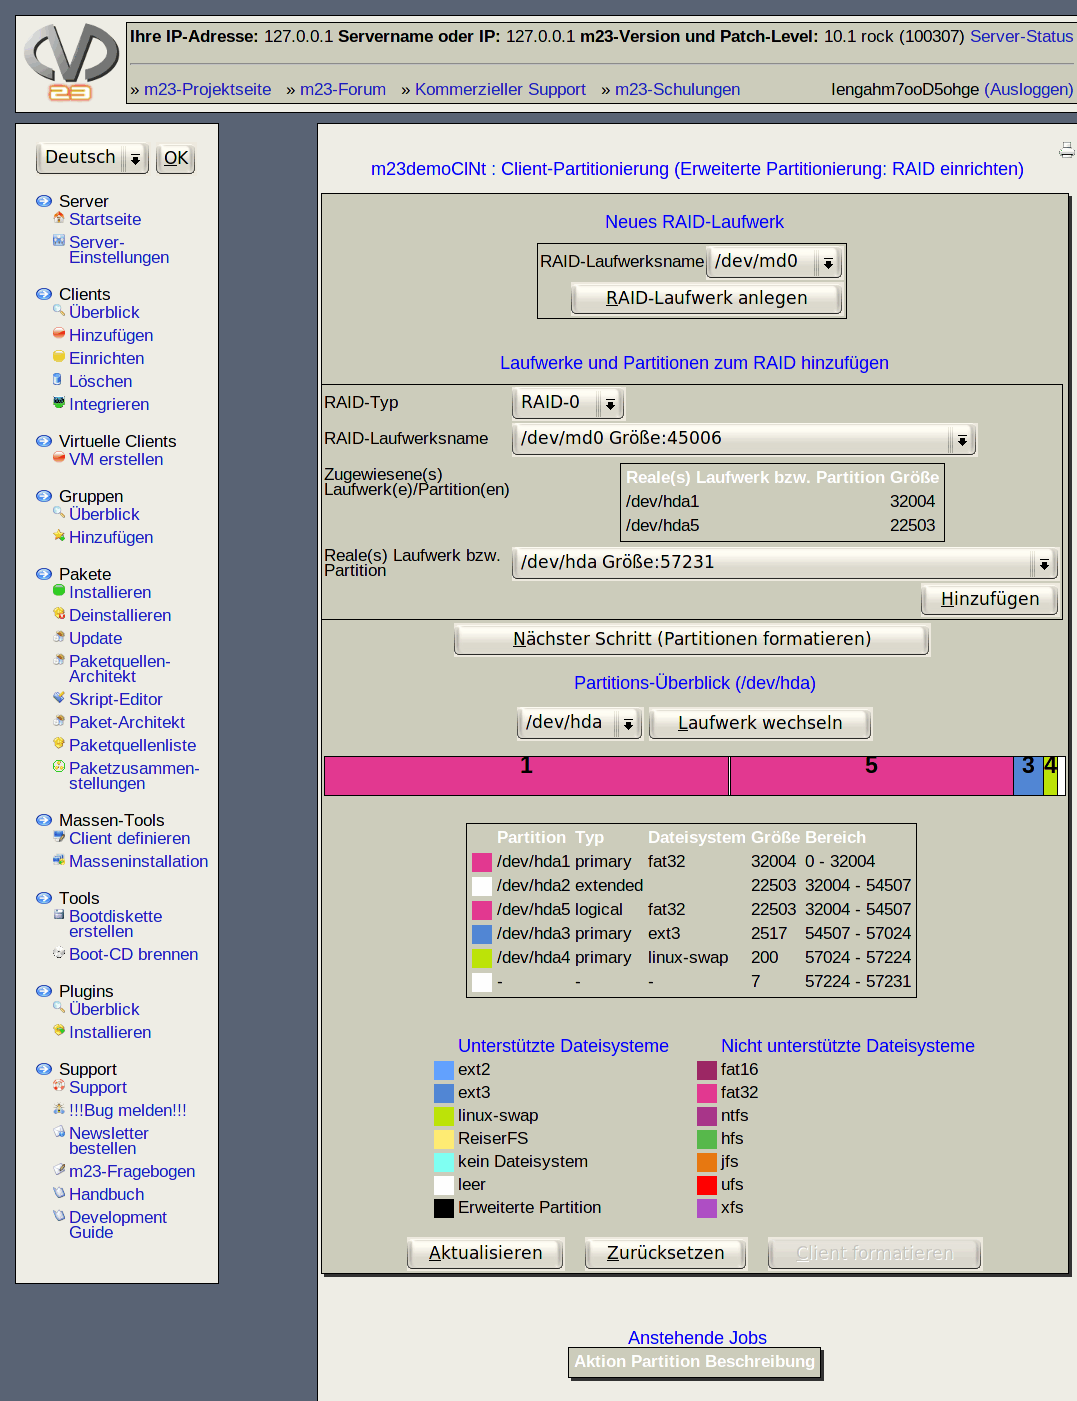
\includegraphics[scale=0.4]{/mdk/doc/manual/screenshots/de/RAID_add.png} \\
In diesem Dialog k�nnen Sie Partitionen oder ganze Laufwerke zu Software-RAIDs zusammenfassen. m23 bzw. das Programm mdadm unterst�tzen die RAID-Level 0, 1, 4, 5, 6 und 10, die jeweils unterschiedliche Vor- und Nachteile im Bezug auf erzielten Geschwindigkeitszuwachs und Ausfallsicherheit bieten. F�r weitere Informationen zu RAIDs lesen Sie bitte die Wikipedia-Seite http://de.wikipedia.org/wiki/RAID. Sie k�nnen mehrere RAIDs pro Client anlegen und dann zur Installation des Betriebssystems, der Swap-Partition etc. benutzen. Lesen Sie bitte den Hinweis, wenn Sie das Betriebssystem auf einem RAID-Laufwerk installieren wollen.\\
\subsection{Schrittweises Vorgehen zum Anlegen eines RAIDs}
\begin{enumerate}
\item \textbf{Anlegen des RAID-Laufwerks:} W�hlen Sie aus der Liste \textit{"RAID-Laufwerksname"} einen Namen aus und klicken Sie anschlie�end auf \textit{"RAID-Laufwerk anlegen"}. Dieses Laufwerk ist ein virtuelles Multi-Device.\\
\item \textbf{Hinzuf�gen von Partitionen und Laufwerken:} In dem Kasten \textit{"Laufwerke und Partitionen zum RAID hinzuf�gen"} finden Sie alle ben�tigten Funktionen zum Zuweisen von Partitionen und Laufwerken zu einem RAID. W�hlen Sie dazu den RAID-Typ und das RAID-Laufwerk aus den entsprechenden Listen aus. Sie k�nnen anschlie�end die weiter unten aufgelistete Partition bzw. das Laufwerk aus der Liste \textit{"Reale(s) Laufwerk bzw. Partition"} dem RAID mit einem Klick auf \textit{"Hinzuf�gen"} zuweisen. In der Tabelle \textit{"Zugewiesene(s) Laufwerk(e)/Partition(en)"} sehen Sie die bereits zugewiesenen Laufwerke und Partitionen.\\
\item \textbf{RAID-Erstellung abschlie�en:} Klicken Sie anschlie�end auf \textit{"N�chster Schritt (Partitionen formatieren)"}.\\
\end{enumerate}
\subsection{Hinweis zu RAIDs und Partitionen}
Auf die RAIDs wird durch die \textit{"Multi device"}-Funktion des Linux-Kernels zugegriffen. Die so gebildeten RAID-Laufwerke verhalten sie wie Partitionen und k�nnen nicht weiter partitioniert werden. Die neue Software-RAID-Variante mit Partitionierungsm�glichkeit wird nicht verwendet, um R�ckw�rtskompatibilit�t zu �lteren Kerneln zu gew�hrleisten.\\
\subsection{Hinweis zur Installation von Betriebssystemen auf RAIDs}
Soll das Betriebssystem auf einem RAID-Laufwerk installiert werden, so mu� meistens (au�er bei RAID-1) eine extra Partition, die nicht auf einem RAID-Laufwerk liegt, f�r den Kernel und die Module angelegt werden. F�r diese Partition reicht eine Gr��e von ca. 50 MB aus. Sollte keine Partition mehr frei sein, so klicken Sie bitte solange auf den \textit{Zur�ck}-Knopf Ihres Browsers bis Sie zum Anlegen bzw. L�schen von Partitionen kommen, und legen Sie eine kleine Partition an.\\
